%!TEX root = ../thesis.tex
%*******************************************************************************
%****************************** Fifth Chapter **********************************
%*******************************************************************************
\chapter{High-Resolution CMB Bispectrum Estimator}

% **************************** Define Graphics Path **************************
\ifpdf
    \graphicspath{{Chapter5/Figs/Raster/}{Chapter5/Figs/PDF/}{Chapter5/Figs/}}
\else
    \graphicspath{{Chapter5/Figs/Vector/}{Chapter5/Figs/}}
\fi



\section{Formalism}

\subsection{CMB-BEst formalism}
Recall that the CMB bispectrum estimator for a given template can be written as
\begin{align}
	\hat{f}_{NL} = \frac{1}{N} \sum_{l_j,m_j} \frac{\mathcal{G}^{l_1 l_2 l_3}_{m_1 m_2 m_3} b_{l_1 l_2 l_3}}{C_{l_1} C_{l_2} C_{l_3}} \left[ a_{l_1 m_1} a_{l_2 m_2} a_{l_3 m_3} - \left( \left< a^G_{l_1 m_1} a^G_{l_2 m_2} \right> a_{l_3 m_3} + \text{2\ cyc.} \right)  \right].		\label{eqn:bispectrum_estimator_standard}
\end{align}
Here we omit superscripts $X$ for temperature and polarisation for notational convenience. Even though the formalism in this section will be presented for CMB temperature data only, the method is general and can easily be extended to include polarisation. For estimation of the full covariance matrix $C_{lm,l'm'}$ needed for the linear term, we use ensemble average from Gaussian simulations, as denoted by superscripts $G$ and the bracket $\left<\cdot\right>$.

The normalisation factor is given by
\begin{align}
	N = \sum_{l_j} \frac{h_{l_1 l_2 l_3}^2 b_{l_1 l_2 l_3}^2}{C_{l_1} C_{l_2} C_{l_3}}.
\end{align}

The core part of our estimation routine is the separable mode expansion of shape function;
\begin{align}
	S(k_1, k_2, k_3) := (k_1 k_2 k_3)^2 B(k_1, k_2, k_3) = \sum_{p_j} \alpha_{p_1 p_2 p_3} q_{p_1}(k_1) q_{p_2}(k_2) q_{p_3}(k_3).
\end{align}
Choices for the basis functions $q_p(k)$ are detailed in the next section. Due to the separability, the reduced bispectrum reduces to a compact form of
\begin{align}
	b_{l_1 l_2 l_3} = \sum_{p_j} \alpha_{p_1 p_2 p_3} \int dr \tilde{q}_{p_1}(l_1,r) \tilde{q}_{p_2}(l_2,r) \tilde{q}_{p_3}(l_3,r),
\end{align}
where the \textit{projected} mode functions are defined as
\begin{align}
	\tilde{q}_{p}(l,r) := \frac{2r^\frac{2}{3}}{\pi} \int dk q_p(k) \Delta_l(k) j_l (kr).
\end{align}
Radiative transfer functions $\Delta_l(k)$ and spherical Bessel functions $j_l(kr)$ are denoted the same way as the previous chapter.

Every term appearing in (\ref{eqn:bispectrum_estimator_standard}) except the Gaunt integral is now separable. Using the definition $\mathcal{G}^{l_1 l_2 l_3}_{m_1 m_2 m_3} = \int d^2 \vv{n} Y_{l_1 m_1}(\vv{n}) Y_{l_2 m_2}(\vv{n}) Y_{l_3 m_3}(\vv{n})$, we can render it separable at the cost of introducing an extra integral.

Define the filtered maps as
\begin{align}
	M^{(i)}_p (\vv{n}, r) := \sum_{l,m} \frac{\tilde{q}_p (l,r)}{C_l} a^{(i)}_{lm} Y_{lm} (\vv{n}), \label{def:filtered_maps}
\end{align}
where $a^{(i)}_{lm}$'s are represent the spherical harmonic transform of the $i$th CMB map. For later convenience, we use a convention where the $0$th map corresponds to the observed CMB map. Maps number $1$-$N_{sims}$ are Gaussian simulations. Note that without the factors involving $\tilde{q}$ and $C_l$'s, $M$ is simply equal to the original map in real space. Each mode extracts different anisotropy scales present in the map.

The bispectrum estimator (\ref{eqn:bispectrum_estimator_standard}) reduces to
\begin{align}
	\hat{f}_{NL}^{(i)} = \frac{1}{N} \sum_{p_j} \alpha_{p_1 p_2 p_3} (\beta^{cub,(i)}_{p_1 p_2 p_3} - 3 \beta^{lin,(i)}_{p_1 p_2 p_3}),
\end{align}
where most of the computation required is now contained in the `$\beta$'s, given by
\begin{align}
	\beta^{cub,(i)}_{p_1 p_2 p_3} &:= \int dr \int d^2\vv{n} \; M^{(i)}_{p_1} (\vv{n},r) M^{(i)}_{p_2} (\vv{n},r) M^{(i)}_{p_3} (\vv{n},r),	\label{def:beta_cubic} \\
	\beta^{lin,(i)}_{p_1 p_2 p_3} &:= \frac{1}{N_{sims}} \sum_{j \neq i} \int dr \int d^2\vv{n} \; M^{(j)}_{p_1} (\vv{n},r) M^{(j)}_{p_2} (\vv{n},r) M^{(i)}_{p_3} (\vv{n},r). \label{def:beta_linear}
\end{align}
Here we evaluate $f_{NL}$ estimates for each of the Gaussian simulations $i=1,\cdots,N_{sims}$. Naturally, they are normally distributed with mean zero. Under the null hypothesis that the initial fluctuations are purely Gaussian and there exist no primordial non-Gaussianity, the value of $f_{NL}$ estimated from the observed CMB map is also drawn from the same normal distribution. Any statistically significant deviations from zero would therefore allow us to reject the null hypothesis.

It is important to note that the beta matrices depends only on the choice of mode functions and input map data, and are independent of the theoretical bispectrum considered. Once $\beta^{cub}$ and $\beta^{lin}$ are computed and stored, we may constrain any model of interest by decomposing the template to get $\alpha$, and then simply taking a dot product: $\vv{\alpha} \cdot \vv{\beta} / N$.

The normalisation can also be obtained in a similar fashion;
\begin{align}
	N = \sum_{p_j, p'_j} \alpha_{p_1 p_2 p_3} \Gamma_{p_1 p_2 p_3, p'_1 p'_2 p'_3} \alpha_{p'_1 p'_2 p'_3},
\end{align}
or equivalently, $N = \vv{\alpha}^T \Gamma \vv{\alpha}$. We exploit separability once again to compute the $\Gamma$ matrix;
\begin{align}
	\Gamma_{p_1 p_2 p_3, p'_1 p'_2 p'_3} &:= \int dr \int d\mu \mathcal{P}_{p_1 p'_1}(\mu, r, r') \mathcal{P}_{p_3 p'_3}(\mu, r, r') \mathcal{P}_{p_3 p'_3}(\mu, r, r'), 	\label{def:gamma} 	\\
	\mathcal{P}_{p p'}(\mu, r, r') &:= \sum_l \frac{2l+1}{(8\pi)^{1/3} C_l} \tilde{q}_{p'}(l,r) \tilde{q}_p(l,r') P_l(\mu),
\end{align}
where $P_l(\mu)$'s are the Legendre polynomials.

In summary, CMB-BEst computes the main quantities: $\beta^{cub}$, $\beta^{lin}$, and $\Gamma$. The most computationally expensive part is the linear term $\beta^{lin}$ by a couple orders of magnitude in most cases. Considerable effort has been put to optimise corresponding part of the code, which will be detailed in the following sections.

\subsection{Basis functions} \label{section:basis_functions}

One of the greatest strengths of CMB-BEst lies in its flexibility with the choice of basis functions. Adopting a specialised basis set provides optimised results to specific models of interest, while a more general construction of basis enable wider search of the model space.

First, we observe that the KSW estimator \cite{Komatsu2005} is derives from a simple monomial basis in our method;
\begin{align}
	q_p(k) = k^{p-1}, \;\;\; p = 0, 1, 2, 3.
\end{align}
All three standard templates - local, equilateral, and orthogonal - can be expressed as a sum of separable terms in the form $q_{p_1}(k_1) q_{p_2}(k_2) q_{p_3}(k_3)$. Shape function of the local template, for example, is given by
\begin{align}
	S^{local}(k_1 k_2 k_3) :=& 2A^2 \left[ \frac{k_1^2}{k_2 k_3} + \frac{k_2^2}{k_3 k_1} + \frac{k_3^2}{k_1 k_2}  \right] \\
	=& 2A^2 \left[q_3(k_1)q_0(k_2)q_0(k_3) + q_0(k_1)q_3(k_2)q_0(k_3) + q_0(k_1)q_0(k_2)q_3(k_3) \right],
\end{align}
where $A$ is the primordial power spectrum amplitude. Decomposition coefficients $\alpha_{p_1 p_2 p_3}$ have three non-zero components: $\alpha_{300} = \alpha_{030} = \alpha_{003} = 2A^2$. Coefficients for the equilateral and orthogonal templates can similarly be found.

We set the scalar spectral index $n_s = 1$ for simplicity above. In the presence of non-unit $n_s$, we modify the basis as follows;
\begin{align}
	q_p(k) = k^2 \left[ k_* \left( \frac{k}{k_*} \right)^{(4-n_s)/3} \right]^{p-4}, \;\; p=0,1,2,3. \label{eqn:KSW_basis}
\end{align}
The pivot scale $k_*$ is defined such that the power spectrum evaluates to $A$ at $k=k_*$. Including $k_*$ here ensures that the $q_p(k)$'s have the right units. Note that the prefactor $k^2$ comes from the definition of shape function and is therefore unaffected by $n_s$. We will refer to this choice of mode functions to be the `KSW' basis.

For studying models with linearly spaced, high-frequency oscillation, a Fourier-like basis
\begin{align}
	q_0(k) = \sin (\omega k), \; q_1(k) = \cos (\omega k),
\end{align}
for a fixed $\omega$ is an appropriate choice. This is in fact equivalent to the method we used to study feature models in Chapter \ref{chapter:CMB_state-4_forecast}. The small size of the basis lets us efficiently constrain theoretical models with given characteristic scale $\omega$. By scanning over a range of $\omega$, or including modes with different values of $\omega$ in the basis, we may also perform a more comprehensive analysis of oscillatory features.

Lastly, we introduce a basis which consists of Legendre polynomials.
\begin{align}
	q_p(k) = P_p(\bar{k}), \;\;\text{where}\;\; \bar{k} = \frac{2k-k_{min}-k_{max}}{k_{max}-k_{min}}.  \label{eqn:Legendre_basis_no_inv_k}
\end{align}
Here we linearly map the range from $k \in [k_{min},k_{max}]$ to $\bar{k} \in [-1,1]$, which is the interval where Legendre polynomials are defined. The number of modes are not bounded; the larger the basis, the more complete coverage of theory space we get.

The Legendre basis has two main advantages over others. First of all, the mode functions are inherently orthogonal, so that $\int_{-1}^{1} d\bar{k} P_{l}(\bar{k}) P_{l'}(\bar{k}) = 0$ whenever $l \neq l'$. This property allows us to greatly simplify the way of decomposing theoretical templates. Given a shape function $S^{(t)} (k_1, k_2, k_3)$, the decomposed coefficients can be found by
\begin{align}
	\alpha^{(t)}_{p_1 p_2 p_3} = \int dk_1 dk_2 dk_3 \; S^{(t)}(k_1, k_2, k_3) q_{p_1}(k_1) q_{p_2}(k_2) q_{p_3}(k_3), \label{def:Legendre_basis}
\end{align}
as long as the modes are normalised appropriately. In practice, we may perform the three one-dimensional integrals one by one, which leads to an efficient and numerically stable algorithm.

Secondly, the Legendre basis enables direct connection to some numerical codes for computing bispectra from various inflationary models, most notably \textsc{Primodal} \cite{Clarke2021}. \textsc{Primodal} is a code for evaluating primordial bispectra from general single-field models. As opposed to other public codes, its output is expressed in terms of the expansion coefficients with respect to the Legendre polynomials. Hence, the result can be directly plugged in to CMB-BEst, creating one fluid pipeline from model to estimation.

As noted in \cite{Clarke2021}, we may augment the base set of Legendre polynomials with one or more particular functions for better description of some bispectrum templates. One solid choice is to add a mode $q(k) = k^{n_s -2}$, orthogonalised with respect to the rest of the basis. This significantly boosts the performance of decomposing local-type bispectra.

Ideally, we would like the $k$ range used in the definition (\ref{def:Legendre_basis}) to be as wide as possible, so that more information from different scales are incorporated in the estimation process. Wider $k$ range, however, also results in lower resolving power because the interval can fit more oscillations of given frequency. Polynomials of higher degrees are necessary to handle the same bispectra. We found that $k_{max}/k_{min} = 1000$ is an overall sweet spot for analysing Planck data.

Throughout the rest of this thesis, we refer to a basis with the $k^{n_s - 2}$ mode and the first 29 Legendre polynomials, totalling 30 modes, defined in the $k$ range with $k_{max}/k_{min}=1000$, as the `Legendre' basis. Any deviation from this set of parameters will be stated explicitly.

\section{Implementation and optimisation}

The CMB-BEst formalism significantly reduces the amount of computation needed for the CMB bispectrum estimation. Obtaining the linear term $\beta^{lin}$ in (\ref{def:beta_linear}), however, is still practically impossible due to its computational complexity unless thoroughly optimised. In this section, we provide details for various aspects of our optimisation process: algorithm design, parallel computing, and data locality improvements. Final specifications and data files used are outlined at the end.

Throughout this section we will treat the functions of interest as discrete arrays. Our notations for indices and their limits are summarised in Table \ref{table:index_conventions}. We adopt simple trapezoidal rule for most numerical integrals, except for the $\mu$ integral in (\ref{def:gamma}) which uses Gauss-Legendre quadrature computed from the public code \textsc{Quadpts} \cite{Hale2013}. Multi-dimensional arrays are stored in the row major order following the \textsc{C} convention. We use the \textsc{libsharp} library \cite{Reinecke2013libsharp} for Spherical Harmonic Transforms (SHTs), and \textsc{Healpix} \cite{Gorski2005healpix} for pixelisation of the sky.

\begin{table}[htbp]
	\caption{Our index conventions for discretised arrays and their sizes.}
	\centering
	\label{table:index_conventions}
	\renewcommand{\arraystretch}{1.5} 
	\begin{tabular}{m{0.1\textwidth}  m{0.1\textwidth}  m{0.7\textwidth}} \toprule
		Index & Range & Description \\
		
		\midrule
		$r$ & $[0, N_r)$ & Line-of-sight integral $r$ grid index. \\
		
		$p, p_j$ & $[0, p_{max})$ & Mode number. $p_j$ is a shorthand for $(p_1, p_2, p_3)$. \\
		
		$i,j$ & $[0, N_{sims}]$ & Map number. Index $i=0$ corresponds to the observed CMB map, while $i>0$ are for simulated Gaussian maps. \\			
		
		$n$ & $[0, N_{pix})$ & Map pixel number. \\ 
		
		$l,m$ & $[0, l_{max})$ & Spherical harmonic multipole moments. Note $-l \le m \le l$. \\
		
		$\mu$ & $[0, N_\mu)$ & Gauss-Legendre quadrature $\mu$ grid index. \\
		
		\bottomrule
	\end{tabular}
\end{table}

\subsection{Algorithm}

Our goal is to compute three key quantities: $\Gamma$ (\ref{def:gamma}), $\beta^{cub}$ (\ref{def:beta_cubic}), and $\beta^{lin}$ (\ref{def:beta_linear}). The matrix $\Gamma$ allows us to find the normalisation factor $N$ for a given theoretical template, while the two $\beta$'s provide the amplitude of $f_{NL}$ for each CMB maps and simulations used, up to normalisation.

In most cases of interest, the bottleneck point of our pipeline is computing the linear term $\beta^{lin}$. Even though the $\Gamma$ matrix computation through (\ref{def:gamma}) grows more rapidly with the number of basis functions ($\propto p_{max}^6$) than the $\beta$'s ($\propto p_{max}^3$), it does not involve operations with high-definition maps and remains subdominant in terms of total cost.

We dedicate this section to explain our algorithm design for $\beta$ computation in detail. The discretised versions of (\ref{def:beta_cubic}-\ref{def:beta_linear}) are given by
\begin{align}
	\beta^{cub}(i, p_1,p_2,p_3) &= \sum_r \sum_n \; M(r, i, p_1, n) \cdot M(r, i, p_2, n) \cdot M(r, i, p_3, n), \\
	\beta^{lin}(i, p_1,p_2,p_3) &= \sum_r \sum_{j \neq i} \sum_n \; M(r, j, p_1, n) \cdot M(r, j, p_2, n) \cdot M(r, i, p_3, n).
\end{align}
The order of indices are chosen such that later calculations have optimal memory layouts. Some integral weights and factors are absorbed into arrays for brevity.

Note that the data arrays for different values of $r$ are completely independent to each other. This provides us a natural way to distribute tasks. We compute and save contributions to $\beta$'s for each $r$ separately. The summation over $r$ is performed in the end. Therefore, throughout the rest of this chapter, we assume that $r$ is fixed and drop the $r$ dependence in descriptions of our algorithms.

The filtered map arrays $M(i,p,n)$ are obtained as follows. A given map $i$ is first transformed in to spherical harmonic coefficients $a^{(i)}(l,m)$s via SHT. We then compute $\tilde{q}_(p,l) * a(i,l,m) / C(l)$ from (\ref{def:filtered_maps}), which is fed into reverse SHT to synthesise the filtered maps.

As a rough guide to the size of each summations, we typically have $N_{sim} \approx 150$ simulations, $p_{max} = 30$ modes, and $N_{pix} = 50,331,648$ pixels. \footnote{This value corresponds to $N_{side} = 2048$ in Healpix. $N_{pix} = 12 N_{side}^2$} Considering the fact that one double-precision array of size $\sim 50$ million pixels takes about 400MB of memory space, this is indeed a task for supercomputers.

Our first and the most straightforward method of computing $\beta$s are outlined in Algorithm \ref{alg:beta_first_attempt}. Computational complexity of each innermost loop is denoted on the right hand side.

\begin{algorithm}[htbp]
	\caption{Computing $\beta$s: the na\"ive method}
	\label{alg:beta_first_attempt}
	\begin{algorithmic}[1] % The number tells where the line numbering should start	
		\State Allocate $M(i,p,n)$
		\Comment{Memory $\sim N_{sims} \cdot p_{max} \cdot N_{pix}$}

		\\
		\For{each map $i$}
			\For{each mode $p$}
			\Comment{$O(N_{sims} \cdot p_{max} \cdot N_{pix}^{3/2})$}
				\State \textbf{compute} $M(i,p,n)$ by SHT
			\EndFor
		\EndFor \Comment{$M(i,p,n)$ ready}
		\\
		
		\For{each map $i$}
			\For{each set of modes $(p_1,p_2,p_3)$}
				\For{each pixel $n$}
				\Comment{$O(N_{sims} \cdot p_{max}^3 \cdot N_{pix})$}
					\State $\beta^{cub}(i, p_1, p_2, p_3) \pluseq M(i,p_1,n) \cdot M(i,p_2,n) \cdot M(i,p_3,n)$
				\EndFor
			\EndFor
		\EndFor

		\\	
		\For{each map $i$}
			\For{each map $j \neq i$}
				\For{each set of modes $(p_1,p_2,p_3)$}
					\For{each pixel $n$}
					\Comment{$O(N_{sims}^2 \cdot p_{max}^3 \cdot N_{pix})$}
						\State $\beta^{lin}(i, p_1, p_2, p_3) \pluseq M(j,p_1,n) \cdot M(j,p_2,n) \cdot M(i,p_3,n)$
					\EndFor
				\EndFor
			\EndFor
		\EndFor

	\end{algorithmic}
\end{algorithm}

Here, we first obtain the filtered maps $M(i,p,n)$ via SHT for each map and modes. The full results are stored in memory. Next, we iterate through each map and set of modes $(p_1, p_2, p_3)$ and sum over each of the map pixels to obtain $\beta^{cub}$ and $\beta^{lin}$. Symmetries in the indices are respected; we only loop over $(p_1,p_2,p_3)$ satisfying $p_1\ge p_2$ for the linear terms, and $p_1\ge p_2\ge p_3$ for the cubic ones.

SHT typically scales as $\propto l_{max}^3$, where $l_{max}$ is the maximum degree of spherical harmonic functions used. The total number of pixels $N_{pix}$ grows $\propto l_{max}^2$ when chosen appropriately for resolution, hence the SHT costs $O(N_{sims}\cdot p_{max} \cdot N_{pix}^{3/2})$. The most expensive part of this algorithm is still the loop where we calculate the linear term, which scales as $O(N_{sims}^2 \cdot p_{max}^3 \cdot N_{pix})$.

Our first major optimisation comes from the observation that we may swap the order of summations to reduce the computation. By precomputing $C(p_1, p_2, n) = \sum_j M(j,p_1,n) \cdot M(j,p_2,n)$, we require one fewer loop over maps for $\beta^{lin}$, leading to a factor of $N_{sims}\sim150$ improvement. Algorithm \ref{alg:beta_second_attempt} shows a pseudocode for this method.

\begin{algorithm}[htbp]
	\caption{Computing $\beta$s: optimised for computation}
	\label{alg:beta_second_attempt}
	\begin{algorithmic}[1] % The number tells where the line numbering should start	
		\State Allocate $M(i,p,n)$ \Comment{Memory $\sim N_{sims} \cdot p_{max} \cdot N_{pix}$}
		\State Allocate $C(p_1,p_2,n)$ \Comment{Memory $\sim p_{max}^2 \cdot N_{pix}$}
		\\
		\For{each map $i$}
			\For{each mode $p$}
				\Comment{$O(N_{sims} \cdot p_{max} \cdot N_{pix}^{3/2})$}
				\State \textbf{compute} $M(i,p,n)$ by SHT
			\EndFor
		\EndFor \Comment{$M(i,p,n)$ ready}
		\\
		\For{each map $j$}
			\For{each pair of modes $(p_1,p_2)$}
				\For{each pixel $n$}
					\Comment{$O(N_{sims} \cdot p_{max}^2 \cdot N_{pix})$}
					\State $C(p_1,p_2,n) \pluseq M(j,p_1,n) \cdot M(j,p_2,n)$
				\EndFor
			\EndFor
		\EndFor \Comment{$C(p_1,p_2,n)$ ready}
		\\
		\For{each map $i$}
			\For{each set of modes $(p_1,p_2,p_3)$}
				\For{each pixel $n$}
					\Comment{$O(N_{sims} \cdot p_{max}^3 \cdot N_{pix})$}
					\State $\beta^{cub}(i, p_1, p_2, p_3) \pluseq M(i, p_1, n) \cdot M(i, p_2, n) \cdot M(i, p_3, n)$
					\State $\beta^{lin}(i, p_1, p_2, p_3) \pluseq C(p_1, p_2, n) \cdot M(i, p_3, n)$
				\EndFor
			\EndFor
		\EndFor
	\end{algorithmic}
\end{algorithm}

Note that the resulting sum fo $\beta^{lin}$ includes an unwanted contribution from the case where $j=i$, since $C(p_1,p_2,n)$ is obtained by summing over all maps. Thankfully, this extra contribution is exactly equal to the cubic term. We just have to subtract $\beta^{cub}$ from the total sum to get the correct value of $\beta^{lin}$.

We shaved off a whole loop at the cost of extra memory usage. For our purposes $N_{sims} ~ 150 > \cdot p_{max} = 30$, so the additional space required for $C(p_1,p_2,n)$ is relatively small compared to $M(i,p,n)$. The symmetry in $p_1$ and $p_2$ also means that we only need to store $p_{max}(p_{max}+1)/2$ maps instead of $p_{max}^2$ for $C$.

Our next challenge is the amount of memory required to save $M(i,p,n)$: $\sim 1.8$TB for the parameters mentioned above, which is quite significant. Though it is not impossible to find supercomputing systems which can accommodate such large arrays, reduction in memory usage would be highly beneficial. We seek to achieve it while keeping the overall computational complexity to be $O(N_{sims} \cdots p_{max}^3 \cdots N_{pix})$ as before.

We observe that most summations are done for a single map $i$. The array $C(p_1,p_2,n)$ is required to be computed before the main loop for $\beta^{lin}$, but otherwise there are no `mixing' between the maps. We exploited this fact to develop Algorithm \ref{alg:beta_third_attempt}.

\begin{algorithm}[htbp]
	\caption{Computing $\beta$s: fast and memory efficient}
	\label{alg:beta_third_attempt}
	\begin{algorithmic}[1] % The number tells where the line numbering should start	
		\State Allocate $m(p,n)$ \Comment{Memory $\sim p_{max} \cdot N_{pix}$}
		\State Allocate $C(p_1,p_2,n)$ \Comment{Memory $\sim p_{max} \cdot p_{max} \cdot N_{pix}$}
		\\
		\For{each map $i$}
			\For{each mode $p$}
				\Comment{$O(N_{sims} \cdot p_{max} \cdot N_{pix}^{3/2})$}
				\State \textbf{compute} $M(i,p,n)$ by SHT and store in $m(p,n)$
			\EndFor
			\\
			\For{each pair of modes $(p_1,p_2)$}
				\For{each pixel $n$}
				\Comment{$O(N_{sims} \cdot p_{max}^2 \cdot N_{pix})$}
					\State $C(p_1,p_2,n) \pluseq m(p_1,n) \cdot m(p_2,n)$
				\EndFor
			\EndFor
		\EndFor
		\Comment{$C(p_1,p_2,n)$ ready}
		\\
		\For{each map $i$}
			\For{each of mode $p$}
				\Comment{$O(N_{sims} \cdot p_{max} \cdot N_{pix}^{3/2})$}
				\State \textbf{compute} $M(i,p,n)$ by SHT and store in $m(p,n)$
			\EndFor
			\\
			\For{each set of modes $(p_1,p_2,p_3)$}		\label{alg:thrid_attempt_main_loop}	
				\For{each pixel $n$}
					\Comment{$O(N_{sims} \cdot p_{max}^3 \cdot N_{pix})$}	
					\State $\beta^{cub}(i, p_1, p_2, p_3) \pluseq m(p_1,n) \cdot m(p_2,n) \cdot m(p_3,n)$
					\State $\beta^{lin}(i, p_1, p_2, p_3) \pluseq C(p_1, p_2, n) \cdot m( p_3, n)$
				\EndFor
			\EndFor
		\EndFor
	\end{algorithmic}
\end{algorithm}

Algorithm \ref{alg:beta_third_attempt} dramatically reduces the amount of memory required, at the cost of doubling the SHTs for computing $M(i,p,n)$s. The first time through, SHT results from each map are used to find $C(p_1,p_2,n)$. After a full loop over maps we have $C(p_1,p_2,n)$ ready, another set of SHTs for each map allows us to obtain the $\beta$'s.

SHTs have subdominant contribution to the total computation time even after becoming doubled in number. One of the main strengths of Algorithm \ref{alg:beta_third_attempt} is that both the memory and computation time scale linearly with the number of simulations used, $N_{sims}$. In the future when a larger number of Gaussian simulations are required to acquire a more accurate estimate of the linear term, it is straightforward to adapt our method accordingly.

We choose Algorithm \ref{alg:beta_third_attempt} to be our main method of computing $\beta$'s for CMB-BEst.

\subsection{Parallel computing}

% Do I need more computing related references here maybe?

In order to fully benefit from the modern computer architecture, parallel computing is a must. In this section, we outline how CMB-BEst was parallelised for optimal performance on supercomputers.

Following \cite{Jeffers2016intel}, we discuss parallelism in three different levels: domain, thread, and data. They mostly correspond to nodes, cores, and registers in modern computer clusters. Each level has distinct characteristics which make them ideal for different parallelisation techniques. We make the full use of each level in our methodology.

\textit{Domain} parallelism refers to dividing the task into many domains where each domain entails heavy computation, while having limited data communication between them. Since the domains are largely independent, Message Passing Interface (MPI) is a suitable tool for parallelisation. MPI is a communication protocol where many instances (`ranks') of the same code may transfer data while running separately from each other. A perfect example of domain parallelism in CMB-BEst would be our line-of-sight integration over $r$. Almost no data are shared between different $r$s, despite the heavy computational cost from map operations within each domain. CMB-BEst therefore scales well with the number of MPI ranks.

\textit{Thread} parallelism opportunities arise when there are many independent computational tasks on a single set of data. Most modern supercomputers use multi-core processors. Each core, or processing units, can run one or more threads, executing instructions independently from each other while sharing memory space. Note that MPI would not be as effective here due to the large amount of data sharing needed; ranks have to either continuously communicate with each other, or store individual copies of the data. This type of parallelism is extremely common in many applications, including SHTs and map integrations in CMB-BEst. Open Multi-Processing (OpenMP) is one of the most popular implementations of multi-threading publicly available. We utilise the \textsc{C} OpenMP interface in our code. 

\textit{Data} parallelism applies when same arithmetic operations are applied to multiple data items, ideally adjacent in memory space. This type of parallel processing is called SIMD: single instruction, multiple data. Many procedures involving large arrays fall into this category. We use Advanced Vector Extensions (AVX) supported by Intel processors to exploit data parallelism in CMB-BEst, especially for operations involving large (filtered) map arrays. In particular, Intel's Xeon Phi series implement AVX-512, where 512-bit registers hold up to 8 double-precision floating numbers. A single instruction can be applied on all of them at once in a single clock cycle, providing a major boost to computation speed. We explicitly align large arrays in memory for optimal vectorisation performance.

Table \ref{table:three_levels_of_parallelism} summarises discussions in this section.

\begin{table}[h]
	\caption{Three levels of parallelism utilised in CMB-BEst. The levels and characteristics are chosen based on \cite{Jeffers2016intel}.}
	\centering
	\label{table:three_levels_of_parallelism}
	\renewcommand{\arraystretch}{1.5} 
	\begin{tabular}{m{0.12\textwidth}   m{0.35\textwidth}   m{0.15\textwidth}   m{0.3\textwidth}} \toprule
		 & Characteristics & Methods & Utilisation \\
		
		\midrule
		Domain \newline Parallelism &
		\begin{itemize}[leftmargin=*]
			\item Limited data communication between domains
			\item Heavy computation within the domain
		\end{itemize} &
		MPI &
		\begin{itemize}[leftmargin=*]
			\item Line of sight $r$ integration split into independent tasks
		\end{itemize}  \\
	
		\midrule
		Thread \newline Parallelism &
		\begin{itemize}[leftmargin=*]
			\item Data sharing between threads
			\item High proportion of independent tasks
		\end{itemize} &
		OpenMP &
		\begin{itemize}[leftmargin=*]
			\item SHT
			\item Map patches divided across threads
		\end{itemize}  \\	
	
		\midrule
		Data \newline Parallelism &
		\begin{itemize}[leftmargin=*]
			\item Same operation applied to multiple data items
		\end{itemize} &
		SIMD &
		\begin{itemize}[leftmargin=*]
			\item Map pixel integration vectorised using AVX-512
			\item Data vectors explicitly aligned in memory for optimal performance 
		\end{itemize} \\	
			
		\bottomrule
	\end{tabular}
\end{table}

\subsection{Data locality}

We implemented Algorithm \ref{alg:beta_third_attempt} and profiled using the Intel VTune Amplifier. Our program was found to be memory-bound, which means that its speed is limited mainly by the amount of memory available and the speed of memory access. The CPU speed, rate of the file I/O, and MPI communication all have subdominant contributions in comparison. This is somewhat expected, since our method deals with large map arrays. The number of operations on each data element is small compared to the size of data, causing the CPUs to be `starved' for data to work on most of the time. Our final set of optimisation focusses on improving memory access patterns.

CPUs of most modern computers contain a small amount of memory attached to them called \textit{cache}. Recently used data and instructions are stored in cache memory so that reusing them is more efficient; accessing cache is much faster than loading from the main, larger memory often shared with other CPUs. Cache is often divided into multiple levels. The smallest and fastest is L1 cache, which is the first level a CPU checks for data. When the required data is not stored in L1 cache, a \textit{cache miss} occurs. The system then has to look further down the cache levels to fetch the wanted data, incurring a large time loss. It is therefore crucial to reuse data as many times as possible before it is lost from cache.

Furthermore, the cache `caches' memory locations in units of cache lines, or chunks of memory containing multiple data elements. Accessing memory locally therefore significantly increases the chance of cache hits, boosting overall performance. Array operations, for example, are optimised when they are stored in consecutive memory locations due to this fact.

CMB-BEst has been modified in two ways to improve data locality and memory performance. The first one was simple yet effective; we made sure to initialise large arrays within the same OpenMP construct as the main computation loop. This guarantees the physical memory of array elements to be allocated near the cores where they are going to be used in. Memory access during the main computation loop is therefore much faster than otherwise. Systems with non-uniform memory access (NUMA) especially benefits from this method. For CMB-BEst, we gained 2 times speed-up compared to when a single master thread initialised the entire array.

The second optimisation centres around \textit{cache blocking}, a technique used to maximise data reuse. Let us focus on the main computation loop in Algorithm \ref{alg:beta_third_attempt}:

\begin{algorithmic}
	\For{each set of modes $(p_1,p_2,p_3)$}
		\For{each pixel $n$}
			\State $\beta^{cub}(i, p_1, p_2, p_3) \pluseq m(p_1,n) \cdot m(p_2,n) \cdot m(p_3,n)$
			\State $\beta^{lin}(i, p_1, p_2, p_3) \pluseq C(p_1, p_2, n) \cdot m( p_3, n)$
		\EndFor
	\EndFor
\end{algorithmic}

In every loop over the set of modes $(p_1, p_2, p_3)$, four large arrays are read from memory: $m(p_1,\cdot)$, $m(p_2,\cdot)$, $m(p_3,\cdot)$, and $C(p_1, p_2, \cdot)$. Each of them take up around 400MB of memory. Since their size is greater than the cache storage capacity, data in the front of them are gone from cache by the time a loop over $n$ completes. All four arrays will then have to be loaded from main memory again when the next iteration starts.

Suppose that the map arrays had smaller size and all of them fit in one of the cache levels instead. After one loop iteration over $n$ for $(p_1, p_2, p_3)$, the arrays now remain in cache. Then the next loop on $(p_1, p_2, p_3+1)$ begins, and the arrays $m(p_1,\cdot)$, $m(p_2,\cdot)$, and $C(p_1,p_2,\cdot)$ are required again for computation. They can now be accessed from cache, which saves significant amount of time. We see that each data element is reused multiple times before discarded from cache in this case.

Motivated by these facts, we divide the map array into equally sized blocks so that each patch can now fit inside the cache memory. We restructure the loop as follows.

\begin{algorithmic}
	\For{each block $b$}
		\For{each set of modes $(p_1,p_2,p_3)$}
			\For{each pixel $n'$ in block}
				\State $\beta^{cub}(i, p_1, p_2, p_3) \pluseq m(p_1,n') \cdot m(p_2,n') \cdot m(p_3,n')$
				\State $\beta^{lin}(i, p_1, p_2, p_3) \pluseq C(p_1, p_2, n') \cdot m( p_3, n')$
			\EndFor
		\EndFor
	\EndFor
\end{algorithmic}

The new pixel numbers are calculated as $n' = B \cdot b + n$, where $B$ is the size of each block and $0 \le n < B$. We have not changed the total number of arithmetic operations required, so the computational complexity remains constant. Meanwhile, data locality within each block is greatly improved, as each of the blocked arrays are now small enough to fit in cache. Each data element is accessed in closer succession temporarily as well.

One caveat here is that having too many blocks may degrade performance. There exist non-negligible overhead coming from an extra \textit{for} loop and the OpenMP construct used over $n'$. The block size divided by number of cores should not be smaller than the size of cache lines either. The optimal size of cache blocks depends on the memory architecture of the processor used. This often needs to be found empirically.

Figure (\ref{fig:cache_block_optimisation}) shows how runtime of a small test code varies with the number of cache blocks used. The code was run on the Intel Gold 6154 processor, which is an 18-core high performance chip with total L1, L2, and L3 cache memory sizes of 1.125MiB, 18MiB, and 24.74MiB, respectively \cite{intel_data_sheet}. Even though some parameters such $N_{sims}$ are tuned down for faster testing, this is representative of the full computation.

\begin{figure}[htbp!] 
	\centering    
	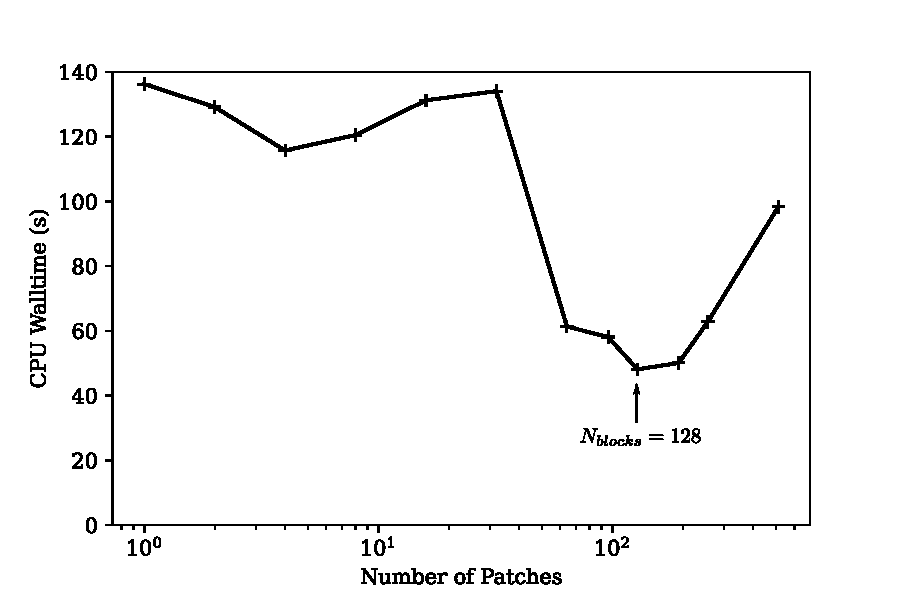
\includegraphics[width=0.8\textwidth]{cache_block_optimisation_annotated.pdf}
	\caption[Cache block optimisation]{Cache block optimisation. Total wall time of a test code for computing $\beta$s was measured while varying the number of cache blocks used. Having 128 blocks is optimal for the 18-core Intel Gold 6154 processor.}
	\label{fig:cache_block_optimisation}
\end{figure}

We observe that having 128 blocks are optimal in this case. Each block now contains about 400,000 elements and takes up 3MiB of memory. Six and eight such blocks may fit in L2 and L3 cache. Compared to the code without any cache blocking, we gain roughly three times speed-up.

Algorithm \ref{alg:beta_final_algorithm} summarises our final implementation of $\beta$ computation code, now with cache blocking and OpenMP construct indicators.

\begin{algorithm}[htbp]
	\caption{Computing $\beta$s: our final implementation}
	\label{alg:beta_final_algorithm}
	\begin{algorithmic}[1] % The number tells where the line numbering should start	
		\State Allocate $m(p,n)$ 
		\State Allocate $C(p_1,p_2,n)$ 
		\\\Comment{Both initialised within OpenMP construct over $n$}

		\For{each map $i$}
		\For{each mode $p$}
		\State \textbf{compute} $M(i,p,n)$ by SHT and store in $m(p,n)$
		\Comment{OpenMP within SHT}
		\EndFor
		\\
		\For{each block $b$}
		\For{each pair of modes $(p_1,p_2)$}
		\For{each pixel $n'$ in block}
		\Comment{OpenMP \textit{for} construct}
		\State $C(p_1,p_2,n') \pluseq m(p_1,n') \cdot m(p_2,n')$
		\EndFor
		\EndFor
		\EndFor
		\EndFor
		\Comment{$C(p_1,p_2,n)$ ready}
		\\
		\For{each map $i$}
		\For{each of mode $p$}
		\State \textbf{compute} $M(i,p,n)$ by SHT and store in $m(p,n)$
		\Comment{OpenMP within SHT}
		\EndFor
		\\
		\For{each block $b$}
		\For{each set of modes $(p_1,p_2,p_3)$}		
		\For{each pixel $n'$ in block}
		\Comment{OpenMP \textit{for} construct}
		\State $\beta^{cub}(i, p_1, p_2, p_3) \pluseq m(p_1,n') \cdot m(p_2,n') \cdot m(p_3,n')$
		\State $\beta^{lin}(i, p_1, p_2, p_3) \pluseq C(p_1, p_2, n') \cdot m( p_3, n')$
		\EndFor
		\EndFor
		\EndFor
		\EndFor
	\end{algorithmic}
\end{algorithm}

\section{Validation}

CMB bispectrum estimation is not only computationally challenging but also prone to numerical instabilities unless implemented carefully. We invested considerable amount of time after the development of CMB-BEst in validating various aspects of the code. We highlight some of our validation efforts in this section, checking consistency within the program itself (section \ref{section:internal_consistency}) and against existing codes such as Modal \cite{Fergusson2012} (section \ref{section:consistency_with_Planck}).

\subsection{Internal consistency checks} \label{section:internal_consistency}

CMB-BEst is a general code where one can freely choose a set of basis functions. Two of our main options are the `KSW' basis (\ref{eqn:KSW_basis}) and `Legendre' basis (\ref{eqn:Legendre_basis_no_inv_k}, augmented with $q(k)=k^{n_s-2}$), as discussed previously in Section \ref{section:basis_functions}. Both basis sets can cover the standard templates: local, equilateral, and orthogonal (see e.g., \cite{PlanckCollaboration2013} for definitions). The KSW basis provides an exact form to the three templates by choosing appropriate powers of $k$ as its basis elements. On the other hand, the templates are expanded in terms of separable Legendre polynomials up to some fixed degree $p_{max}$ for the Legendre basis. As long as $p_{max}$ is sufficiently large, most smooth bispectrum shapes can be represented accurately. 

Our first consistency check is shown in Figure \ref{fig:map_by_map_Legendre_KSW}, where we compare the $f_{NL}$ estimates from the Planck 2018 CMB map and 140 full focal plane (FFP10) realistic Gaussian simulations \cite{PlanckCollaboration2015simulations}. We use CMB maps obtained through the SMICA component separation method \cite{Cardoso2008component, PlanckCollaboration2013ComponentSeparation}. On the left hand side are scatter plots of $f_{NL}$ values obtained using each of the two basis sets. In an ideal case where the two estimates are identical for every test maps, all the points would lie on a straight line given by $y=x$. Drawn in dashed red line is the best linear fit to the data. Its slope, intercept, and the $R$-squared value are annotated below. On the right is a more detailed plot of computed $f_{NL}$ for each map.

\begin{figure}[htbp!] 
	\centering 
	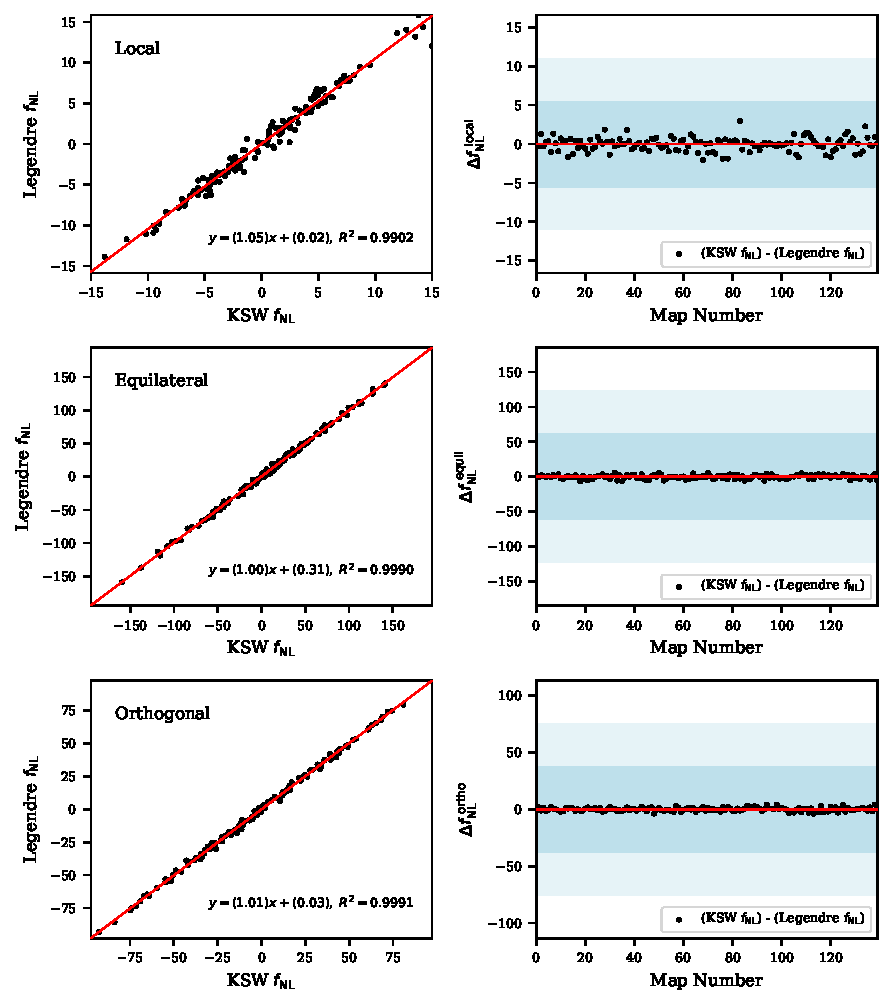
\includegraphics[width=\textwidth]{map_by_map_Legendre_KSW.pdf}
	\caption{Map-by-map comparison of $f_{NL}$ estimates for standard templates, evaluated using each of the KSW and Legendre basis sets. Planck 2018 CMB map and 140 FFP10 simulations have been used, each representing a single point on the scatter plot shown left. Details of the linear best-fit to data (red dashed) is annotated below. On the right hand side shows a plot of $f_{NL}$ values for each map. In the ideal case where the two basis sets yield identical results, we should see all the points on $y=x$ for the left plot, and exactly overlapping graphs for the right. For more information on  each of the three theoretical templates used, see e.g., \cite{PlanckCollaboration2013}.}
	\label{fig:map_by_map_Legendre_KSW}
\end{figure}

We see that results from the two different sets of basis are in good agreement. The $R$-squared value of the linear fit is greater than $0.99$ for Local, and $0.999$ for Equilateral and Orthogonal shapes. The intercepts are also near zero, meaning that the lensing-ISW bias has been subtracted off consistently for both cases. A closer look at the  individual map estimates reveals no systematic discrepancies across the shapes.

Validates: cubic/linear term working well, Gaussian dist checked, decomp routine for Legendre, different primordial modes gets projected and combines well!

%Quick derivation of optimality of the bispectrum estimator?
Estimation part:
+ Slight scatter in local -> k ratio 2000 plot
- Sample vs theoretical variance.
- Sample versus Theory covariance checks.
- Expected chi-square distribution etc.
Convergence part:
- Convergence epsilon definition
- Standard templates convergence epsilons
+ Legendre - pmax=29 vs 30 for trio
- Legendre - constant feature models part. Correlation matrix



\begin{figure}[htbp!] 
	\centering    
	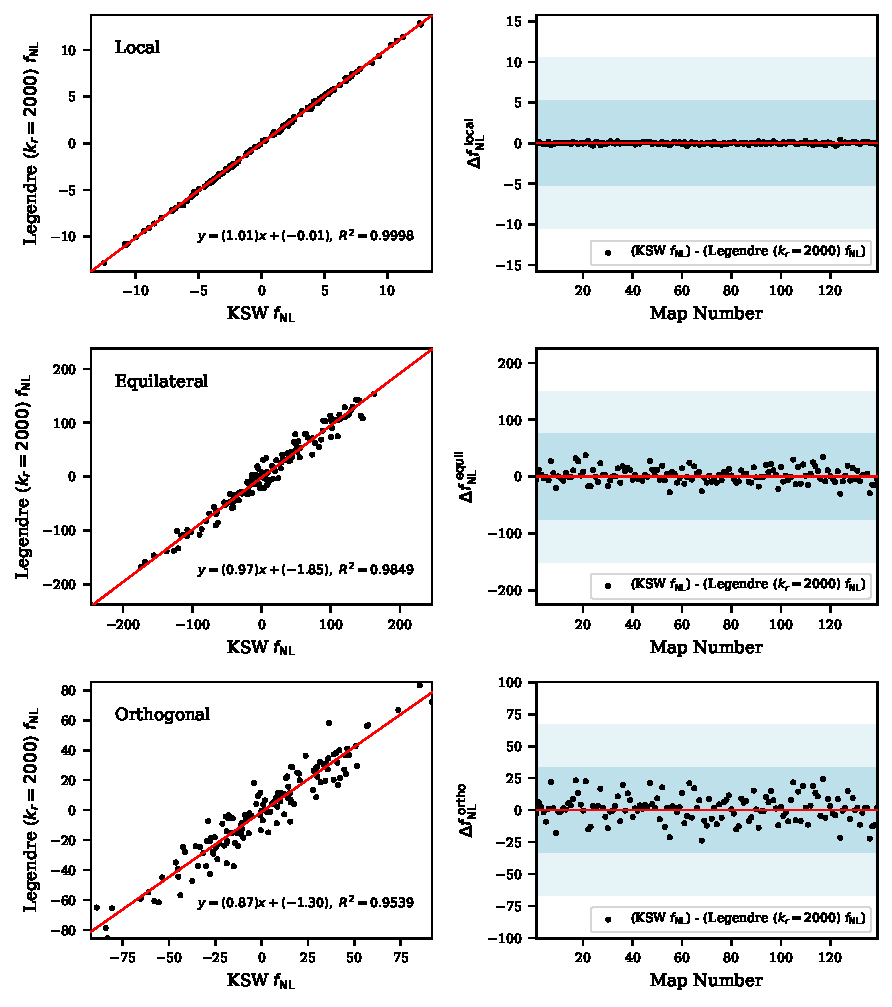
\includegraphics[width=\textwidth]{map_by_map_Legendre_KSW_k_ratio_2000.pdf}
	\caption{KSW vs Legendre, k ratio 2000}
	\label{fig:map_by_map_Legendre_KSW_k_ratio_2000}
\end{figure}

\begin{figure}[htbp!] 
	\centering    
	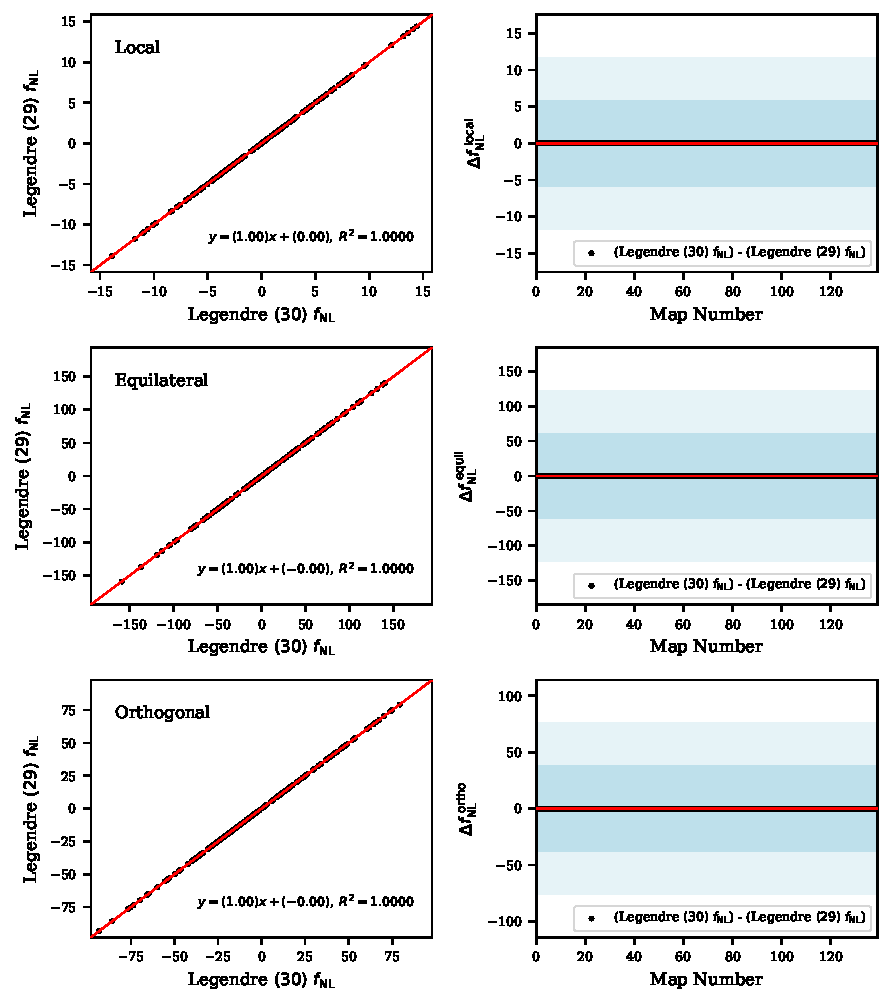
\includegraphics[width=\textwidth]{map_by_map_Legendre_30_29.pdf}
	\caption{Legendre 29 vs 30}
	\label{fig:map_by_map_Legendre_30_29}
\end{figure}

\begin{figure}[htbp!] 
	\centering    
	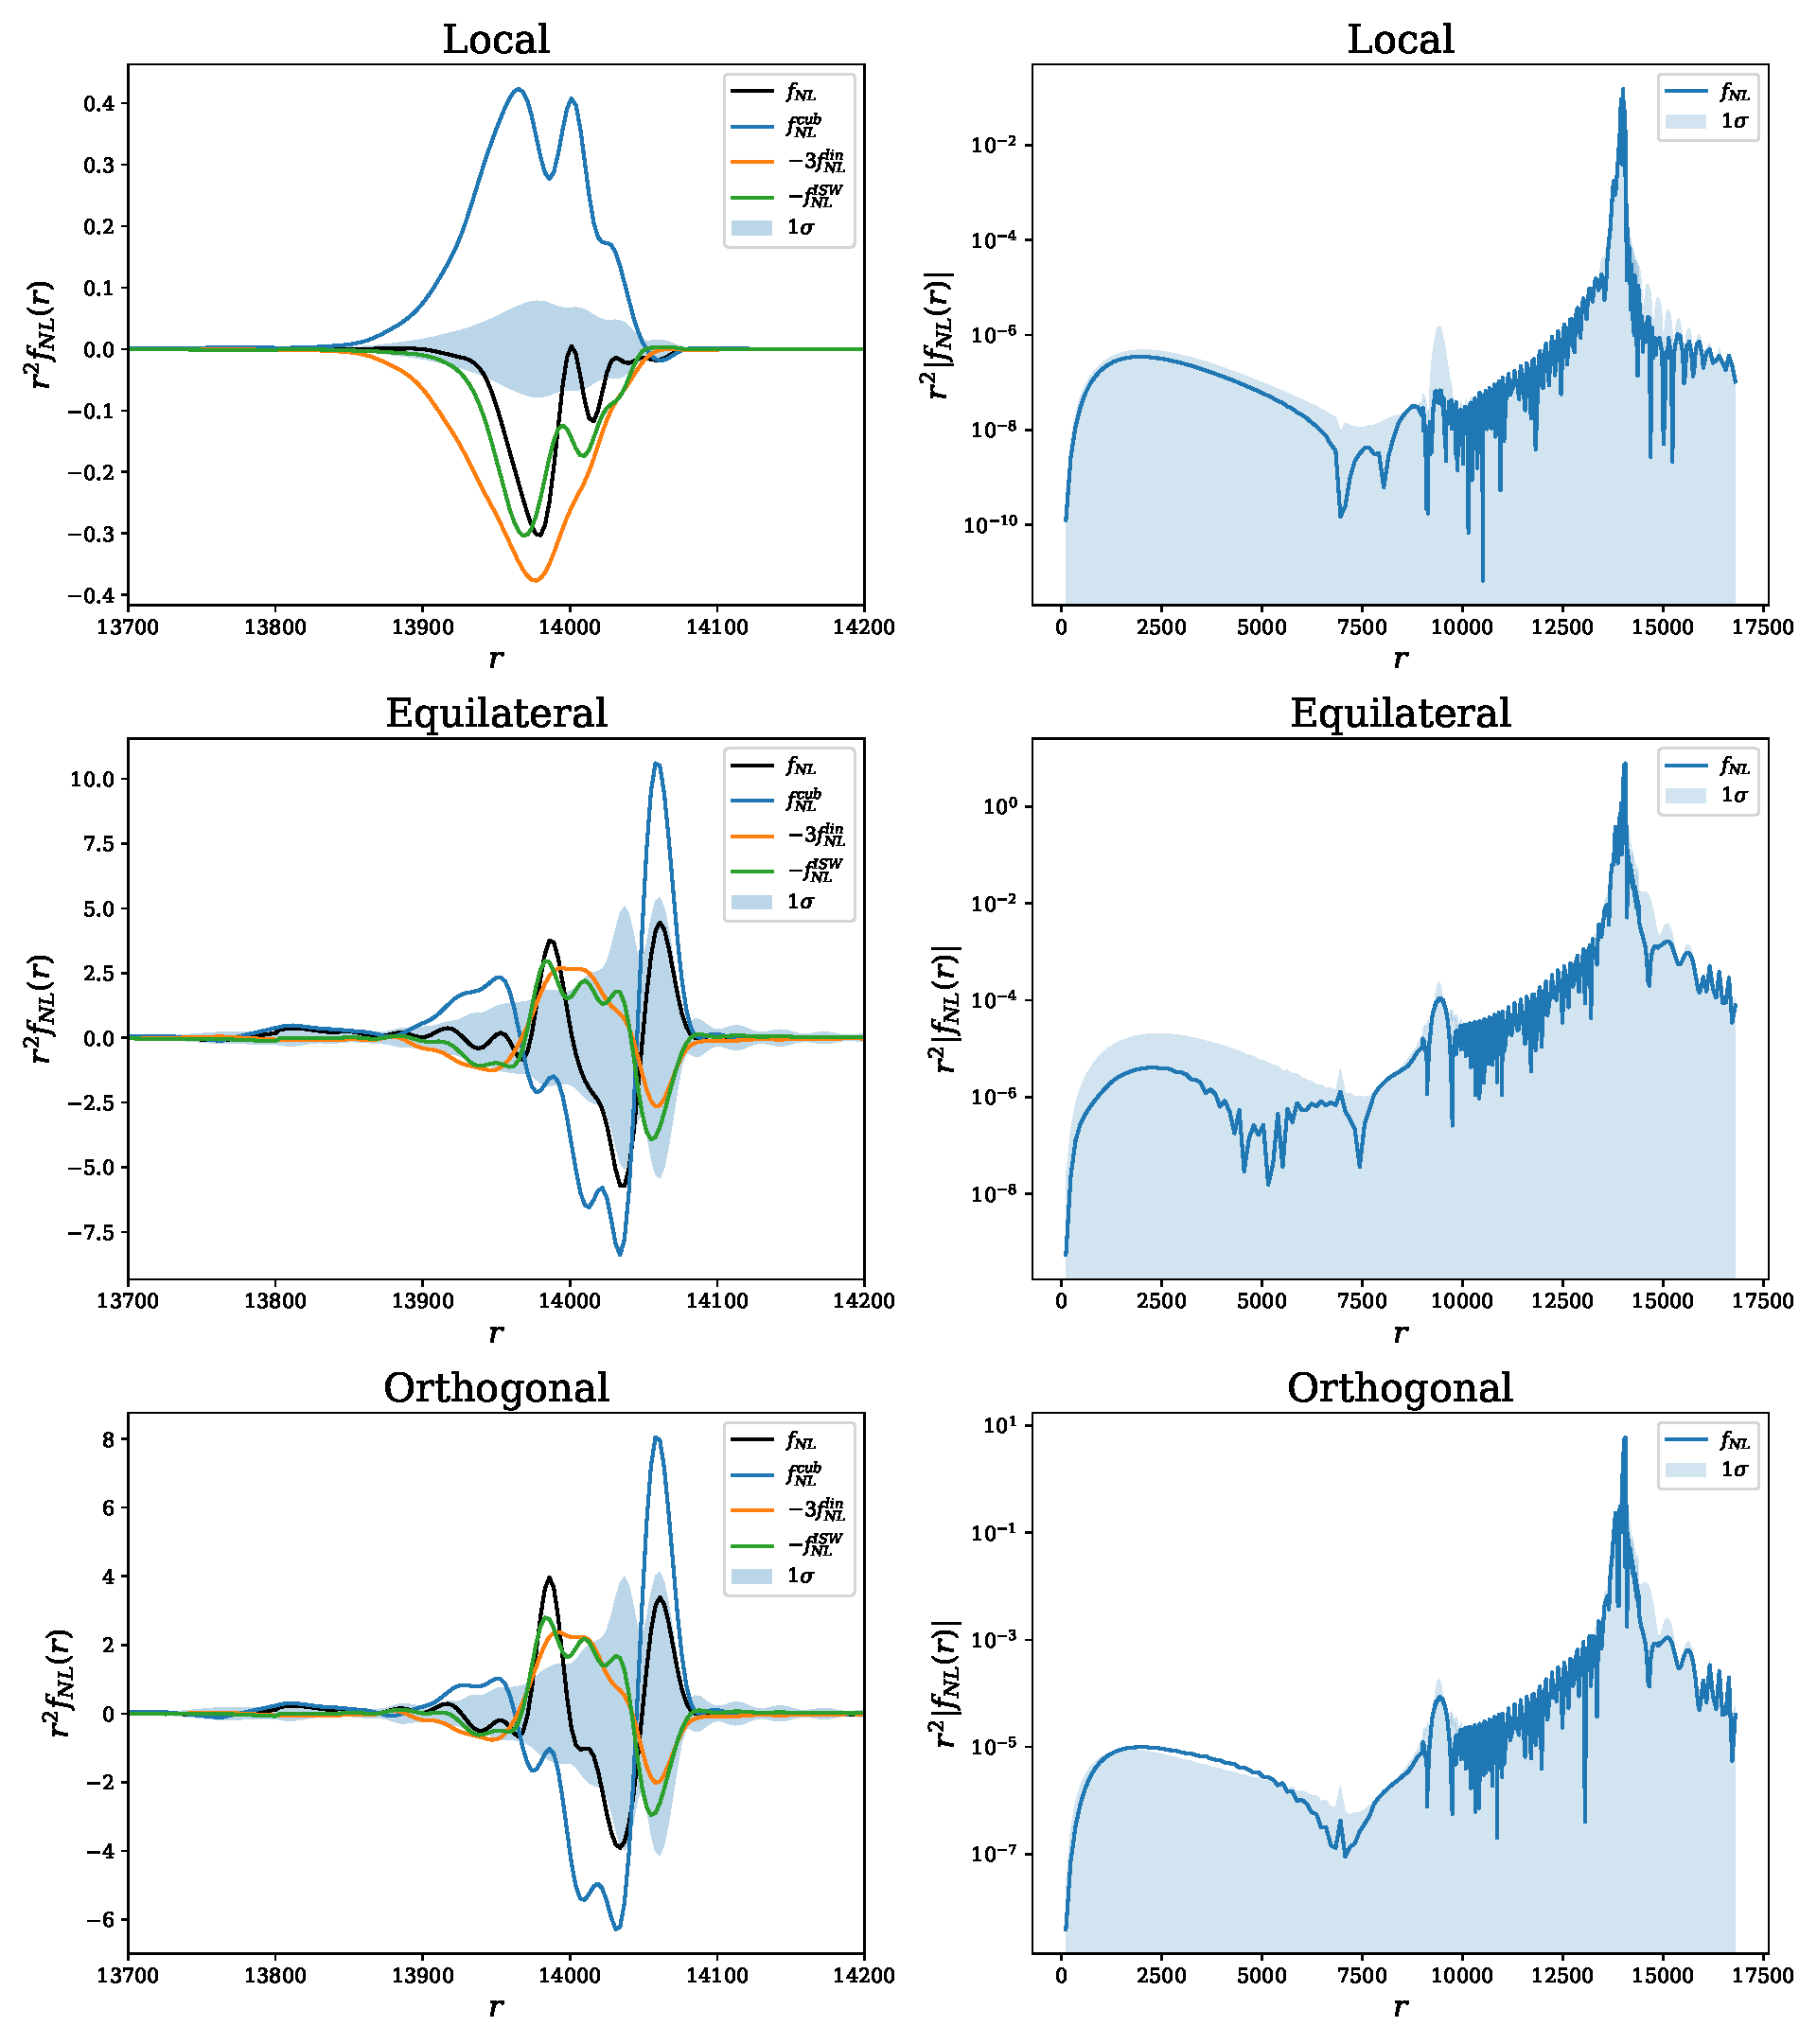
\includegraphics[width=\textwidth]{trio_r_dependence.pdf}
	\caption{Trio r dependence}
	\label{fig:trio_r_dependence}
\end{figure}

\subsection{Consistency with Planck} \label{section:consistency_with_Planck}

+ KSW vs Leg vs Modal table
+ Map-by-map plot for Leg vs Modal Trio
- Plot for Leg vs Modal, fNL vs frequency plot
- Frequency correlation plot
- Epsilon vs frequency. Primordial convergence vs late-time...

Consistency vs Modal for Planck results.
Discussion on kmin and kmax range


\begin{table}[h]
	\caption{Constraints for the standard templates for the KSW and Legendre basis from CMB-BEst, in comparison with the Planck 2018 analysis \cite{PlanckCollaboration2018}. SMICA temperature map has been used, and the lensing bias has been subtracted.}
	\centering
	\label{table:trio_fNL_comparison_with_planck}
	\renewcommand{\arraystretch}{1.5} 
	\begin{tabular}{lcccc}
		\toprule
		& \multicolumn{2}{c}{CMB-BEst} & \multicolumn{2}{c}{Planck 2018} \\ \cmidrule(lr){2-3} \cmidrule(lr){4-5}
		Template & KSW &  Legendre &  KSW &  Modal \\
		\midrule
		
		Local & $-2.2 \;\pm\; 5.5$ & $-2.0 \;\pm\; 5.9$ & $-0.5 \;\pm\; 5.6$ & $-0.6 \;\pm\; 6.4$ \\
		Equilateral & $17 \;\pm\; 61$ & $15 \;\pm\; 62$ & $7 \;\pm\; 66$ & $34 \;\pm\; 67$ \\
		Orthogonal & $-7 \;\pm\; 38$ & $-9 \;\pm\; 38$ & $-15 \;\pm\; 36$ & $-26 \;\pm\; 43$ \\
		\bottomrule
	\end{tabular}
\end{table}


\begin{figure}[htbp!] 
	\centering    
	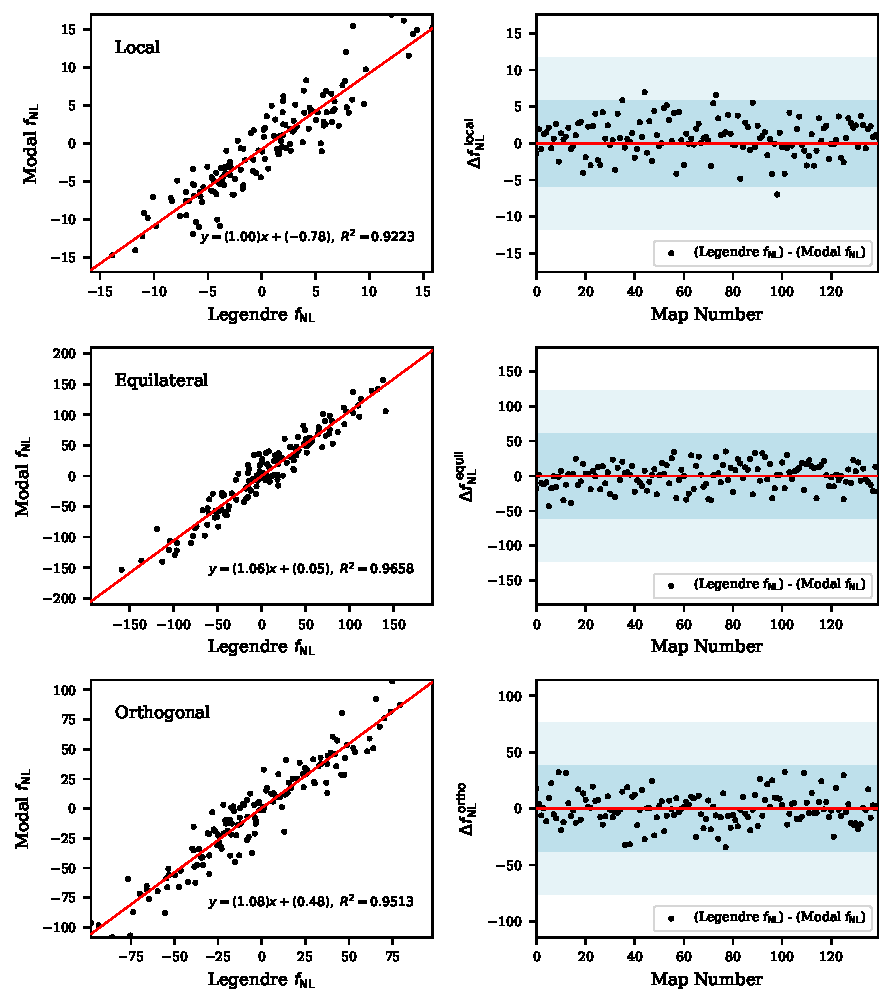
\includegraphics[width=\textwidth]{map_by_map_Legendre_Modal.pdf}
	\caption{Legendre vs Modal}
	\label{fig:map_by_map_Legendre_Modal}
\end{figure}

\begin{figure}[htbp!] 
	\centering    
	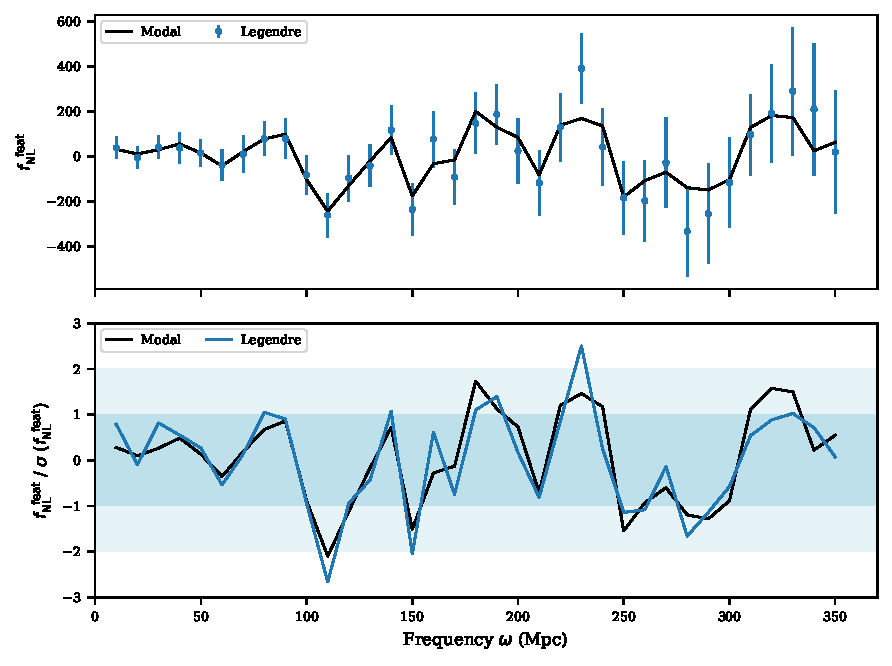
\includegraphics[width=\textwidth]{sine_template_frequency_Legendre_Modal.pdf}
	\caption{Feature model, sine, Legendre vs Modal}
	\label{fig:sine_template_frequency_Legendre_Modal}
\end{figure}

\begin{figure}[htbp!] 
	\centering    
	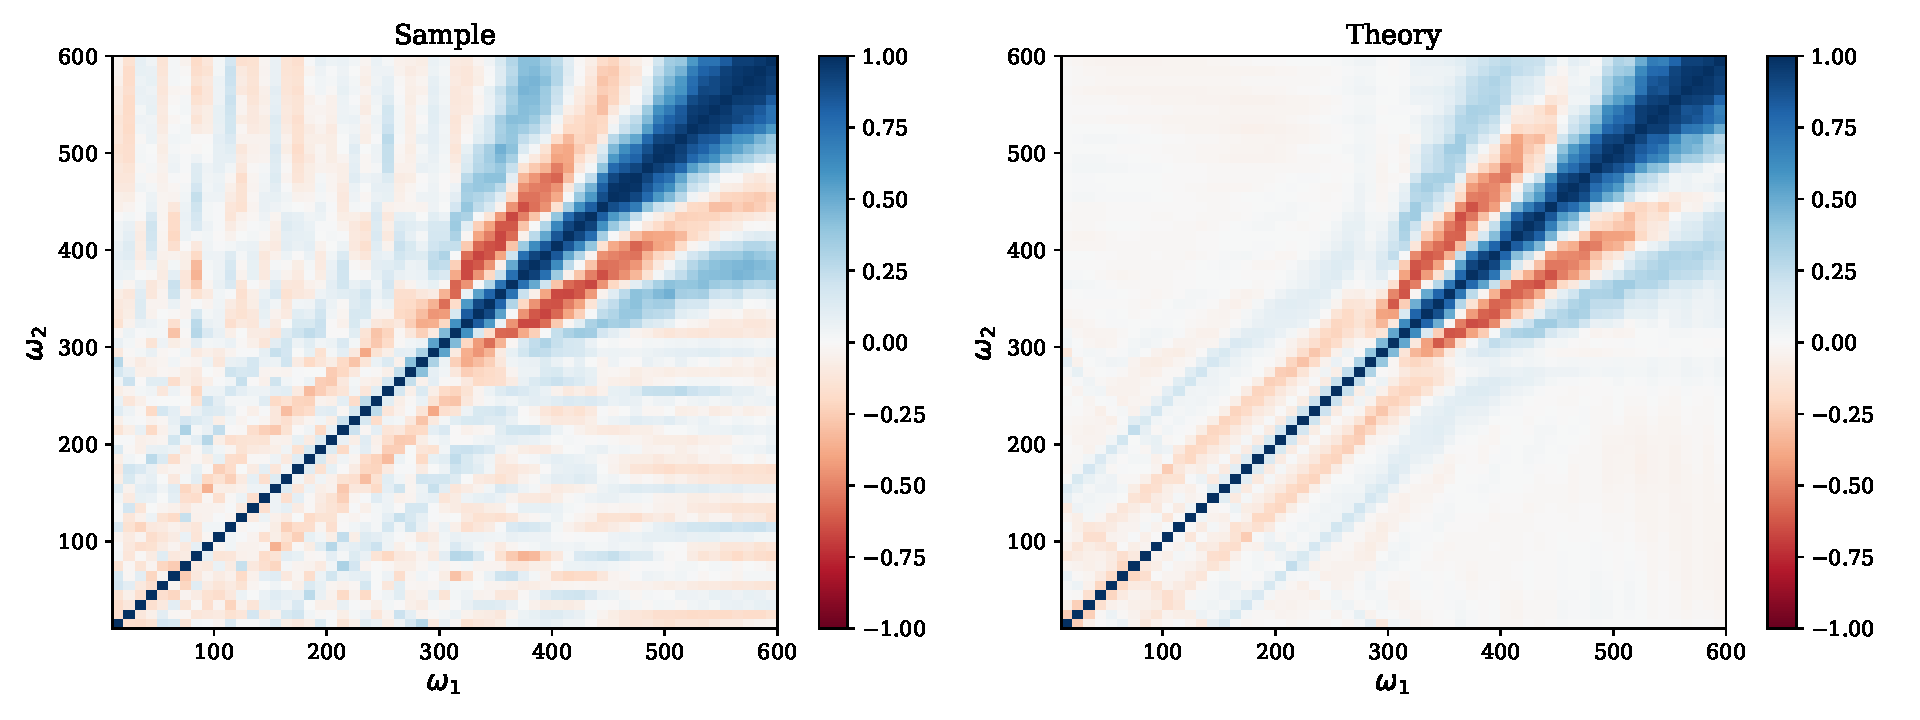
\includegraphics[width=\textwidth]{sine_template_correlations_new.pdf}
	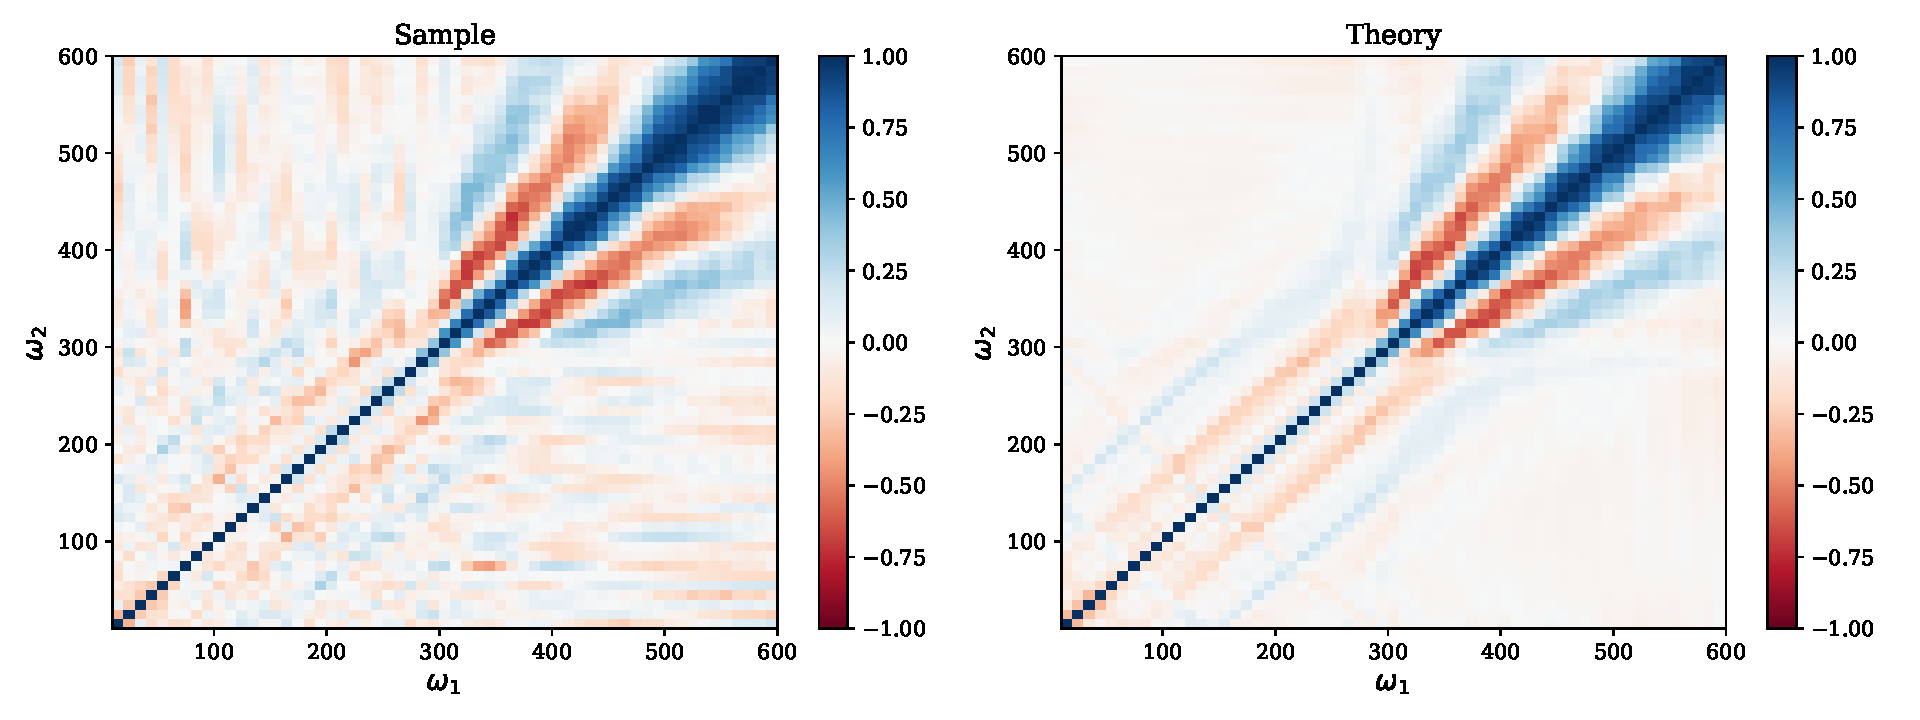
\includegraphics[width=\textwidth]{cosine_template_correlations_new.pdf}
	\caption{Feature model template correlations, sample and theoretical}
	\label{fig:feature_template_correlations}
\end{figure}

\subsection{Proof of concept}

- DBI sound speed constraints
- DBI resonance scan
- tetrapyd decomp? 

\begin{figure}[htbp!] 
	\centering    
	\includegraphics[width=0.9\textwidth]{dbi_sound_speed_scan_annotated.pdf}
	\caption{DBI sound speed scan}
	\label{fig:dbi_sound_speed_scan}
\end{figure}


\subsection{Future work}





% Old table
%\begin{table}[h]
%	\caption{Constraints for the standard templates for the KSW and Legendre basis from CMB-BEst, in comparison with the `Modal' pipeline from Planck 2018 analysis \cite{PlanckCollaboration2018}}
%	\centering
%	\label{table:trio_fNL_comparison_with_planck}
%	\renewcommand{\arraystretch}{1.5} 
%	\begin{tabular}{llrrr}
%		\toprule
%		Template & Estimator &  $f_{NL}^T$ &  $\bar{\sigma}^T$ &  $\sigma^T$ \\
%		\toprule
%		
%		Local & KSW &   -2.2 &      5.5 &      5.3 \\
%		& Legendre &   -2.0 &      5.9 &      5.7 \\
%		& Modal &   -0.6 &      6.4 &      6.1 \\
%		
%		\midrule
%		Equilateral & KSW &   16.7 &     61.1 &     67.7 \\
%		& Legendre &   15.2 &     61.7 &     67.7 \\
%		& Modal &   33.8 &     66.5 &     72.4 \\
%		
%		\midrule
%		Orthogonal & KSW &   -6.9 &     37.6 &     33.7 \\
%		& Legendre &   -8.5 &     38.0 &     33.9 \\
%		& Modal &  -26.5 &     42.8 &     39.3 \\
%		\bottomrule
%	\end{tabular}
%\end{table}
